\documentclass[aspectratio=169]{beamer}

% ==================================================================
% Define custom colors
\definecolor{primarycolor}{RGB}{25, 74, 166} % blue
\definecolor{accentcolor}{RGB}{65, 155, 232} % lighter blue
\definecolor{bluepoli}{RGB}{2, 30, 54}

% ==================================================================
% Apply these colors
\setbeamercolor{normal text}{fg=black, bg=white}
\setbeamercolor{alerted text}{fg=accentcolor}
\setbeamercolor{example text}{fg=accentcolor!80!black}
\setbeamercolor{progress bar}{fg=accentcolor, bg=accentcolor!20}
\setbeamercolor{frametitle}{bg=bluepoli, fg=bluepoli!80!black}
\setbeamercolor{title separator}{fg=bluepoli}

% ==================================================================
% Metropolis customization
\usetheme[sectionpage=none]{metropolis}
\setbeamercolor{background canvas}{bg=black!1.5}
\setbeamercolor{frametitle}{bg=black!1.5,fg=black}
\setbeamertemplate{sections/subsections in toc}[square]
\setbeamertemplate{footline}{
    \centerline{\textcolor{bluepoli}{\rule{0.95\paperwidth}{.3pt}}}
    \vskip2.5pt
    \hskip15pt \tiny Introduction to Matlab \hskip350pt \insertframenumber
    \vskip4pt
}

% ==================================================================
% Images
\usepackage{graphicx}

% ==================================================================
% Colors
\usepackage{color}
\usepackage[dvipsnames]{xcolor}
\usepackage{colortbl}

% ==================================================================
% Code rendering
\usepackage{minted}
% \usemintedstyle{colorful}  % or 'vs', 'github', 'monokai'

% ==================================================================
% TIKZ
\usepackage{tikz}
\usetikzlibrary{positioning,tikzmark}

% ==================================================================
% Highlighting command for math mode
\newcommand{\mathcolorbox}[2]{\tikz[baseline=(char.base)]{
    \node[rectangle, fill=#1!20, inner sep=1pt, rounded corners=2pt] (char) {$#2$};}
}

% ==================================================================
% TITLE
\title{Introduction to MATLAB}
\subtitle{Calcoli di Processo dell' Ingegneria Chimica}
\author[Dinelli, Mehl]{\textbf{Timoteo~Dinelli}}
\institute{
   \inst{} Department of Chemistry, Materials and Chemical Enginering, ``Giulio Natta'', Politecnico di Milano.\\ \\
   \textbf{email}: timoteo.dinelli@polimi.it
}
\date{
    25\textsuperscript{\underline{th}} of September 2025,\\
    02\textsuperscript{\underline{nd}} of October 2025,\\
    07\textsuperscript{\underline{th}} of October 2025.
}

\begin{document}
{
    \setbeamertemplate{footline}{} 
    \begin{frame}{}
        \maketitle
        \begin{tikzpicture}[overlay, remember picture]
            \node[above left=3.6cm and 0.01cm of current page.south east] {
                
\includegraphics[trim=1cm 1cm 5.5cm 1cm, clip=true, width=8cm]{figures/logo.pdf}
            };
        \end{tikzpicture}
    \end{frame}
}

% ==================================================================
% Slides
\begin{frame}{Contacts \& Information}
    \textbf{Professor}: Marco Mehl \\
    \textbf{e-mail}: marco.mehl@polimi.it \\
    \textbf{Office}: Leonardo Campus, Building 6, Department of Chemistry, Materials and Chemical Enginering, ``Giulio Natta'', Politecnico di Milano. \\
    \vskip 1cm
    \textbf{Teacher assistant}: Timoteo Dinelli \\
    \textbf{e-mail}: timoteo.dinelli@polimi.it \\
    \textbf{Office}: Leonardo Campus, Building 6, Department of Chemistry, Materials and Chemical Enginering, ``Giulio Natta'', Politecnico di Milano. \\
\end{frame}

\begin{frame}{Resources}
    \small \alert{Books}:
    \begin{itemize}
        \item[$\blacktriangleright$]
            \href{http://hdl.handle.net/11311/579545}{\footnotesize G., Buzzi Ferraris; Manenti, Flavio. Fundamentals and Linear Algebra for the Chemical Engineer: Solving Numerical Problems.} 

        \item[$\blacktriangleright$]
            \href{http://hdl.handle.net/11311/579546}{\footnotesize G., Buzzi Ferraris; Manenti, Flavio. Interpolation and Regression Models for the Chemical Engineer: Solving Numerical Problems.} 

        \item[$\blacktriangleright$]
            \href{http://hdl.handle.net/11311/663722}{\footnotesize G., Buzzi Ferraris; Manenti, Flavio. Nonlinear Systems and Optimization for the Chemical Engineer: Solving Numerical Problems.}

        \item[$\blacktriangleright$]
            \href{http://hdl.handle.net/11311/1003033}{\footnotesize G., Buzzi Ferraris; Manenti, Flavio. Differential and Differential-Algebraic Systems for the Chemical Engineer: Solving Numerical Problems.}

        \item[$\blacktriangleright$]
            \href{https://www.biblio.com/9780199660346}{\footnotesize J. Nathan Kutz. Data-Driven Modeling and Scientific Computation.}
   \end{itemize}
\end{frame}

\begin{frame}{}
    \begin{itemize}
        \item[$\blacktriangleright$]
            \href{https://www.amazon.it/Data-Driven-Science-Engineering-Learning-Dynamical/dp/1009098489/ref=asc_df_1009098489/?tag=googshopit-21&linkCode=df0&hvadid=560287860614&hvpos=&hvnetw=g&hvrand=14266207767663986773&hvpone=&hvptwo=&hvqmt=&hvdev=c&hvdvcmdl=&hvlocint=&hvlocphy=1008463&hvtargid=pla-1599460130783&psc=1}{\footnotesize Steven L. Brunton; J. Nathan Kutz. Data-Driven Science and Engineering: Machine Learning, Dynamical Systems, and Control.}

        \item[$\blacktriangleright$]
            \href{https://link.springer.com/book/10.1007/978-88-470-5644-2}{\footnotesize A. Quarteroni; R. Sacco; F. Saleri; P. Gervasio. Matematica Numerica.}

        \item[$\blacktriangleright$]
            \href{https://www.amazon.it/Calcolo-Scientifico-Esercizi-problemi-risolti-dp-8847039525/dp/8847039525/ref=dp_ob_title_bk}{\footnotesize A. Quarteroni; F. Saleri; P. Gervasio. Calcolo Scientifico: Esercizi e problemi risolti con MATLAB e Octave.}

        \item[$\blacktriangleright$]
            \href{https://www.ibs.it/calcolo-numerico-applicato-libro-davide-manca/e/9788837116972}{\footnotesize D. Manca. Calcolo numerico applicato.}
    \end{itemize}
    \vskip .5cm
    \small \alert{Online Material}:
    \begin{itemize}
        \item[$\blacktriangleright$]
            \href{https://ocw.mit.edu/courses/10-34-numerical-methods-applied-to-chemical-engineering-fall-2015/pages/syllabus/}{\footnotesize Numerical Methods applied to chemical engineering (MIT).}

        \item[$\blacktriangleright$]
            \href{https://github.com/Titodinelli/Calcoli-di-Processo-dell-Ingegneria-Chimica}{\footnotesize GitHub repository of the practical sessions.}

        \item[$\blacktriangleright$]
            \href{https://it.mathworks.com/help/matlab/getting-started-with-matlab.html}{\footnotesize Matlab online tutorial and documentation.}
    \end{itemize}
\end{frame}

% ==================================================================
% TOC
\begin{frame}
\frametitle{Table of Contents}
    \begin{columns}[t]
        \begin{column}{0.5\textwidth}
            \hypersetup{linkcolor=accentcolor}{\tableofcontents[sections={1-3}]}
        \end{column}
        \begin{column}{0.5\textwidth}
            \hypersetup{linkcolor=accentcolor}{\tableofcontents[sections={4-8}]}
        \end{column}
    \end{columns}
\end{frame}

\section{Introduction}
\subsection{What is programming?}
\begin{frame}{What is programming?}
    \small{
        \begin{itemize}[<+->]
            \item[$\blacktriangleright$]
            The most simple answer is: ``Programming is the \underline{\textbf{act}} or activity of writing computer programs''. In a more general way programming or coding is the act of writing a computer program.

            \item[$\blacktriangleright$]
            A \underline{\textbf{computer program}} is a sequence of instructions that a computer is able to execute.

            \item[$\blacktriangleright$]
            \underline{\textbf{Computer}} in the definition above is any device that is capable of processing code. This could be smartphones, ATMs, the Raspberry Pi, Servers to name a few.
        \end{itemize}

        \pause
        Remember, every time we use smart devices, some code is running in the background. Moving a mouse pointer from one part of your computer screen to the other may seem like a simple task, but in reality, so many lines of code just ran. An act as simple as typing letters into Google Docs leads to lines of code being executed in the background. It’s all code everywhere.
    }
\end{frame}

\subsection{The Natural Language of Computers}
\begin{frame}{The Natural Language of Computers}
    \begin{columns}
        \begin{column}{0.5\textwidth}
            \begin{figure}
                \centering
                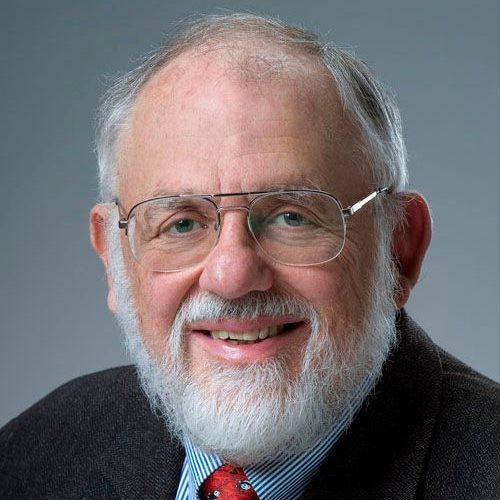
\includegraphics[width=0.85\textwidth]{figures/cleve_moler.jpg}
                \caption{Cleve Barry Moler}
            \end{figure}
        \end{column}

        \begin{column}{0.5\textwidth}
            \small{
                The \underline{\textbf{only}} language understood by a computer is the machine language. A very long list of 0 and 1. However it is a little bit inconvenient to write a series of zeros and ones. So (very smart) people, like the one in the picture, invented what are called programming languages (C/C++, Fortran, python,
                julia, MATLAB, ...).

                \alert{\textbf{N.B.}} Computers aren't very smart, the instructions need to be very precise! Telling a computer what you want it to do is sometimes hard because you have to explain things very carefully and precisely.
            }
        \end{column}
    \end{columns}
\end{frame}

\section{First Steps with MATLAB}
\begin{frame}{MATLAB}
    \begin{figure}
        \centering
        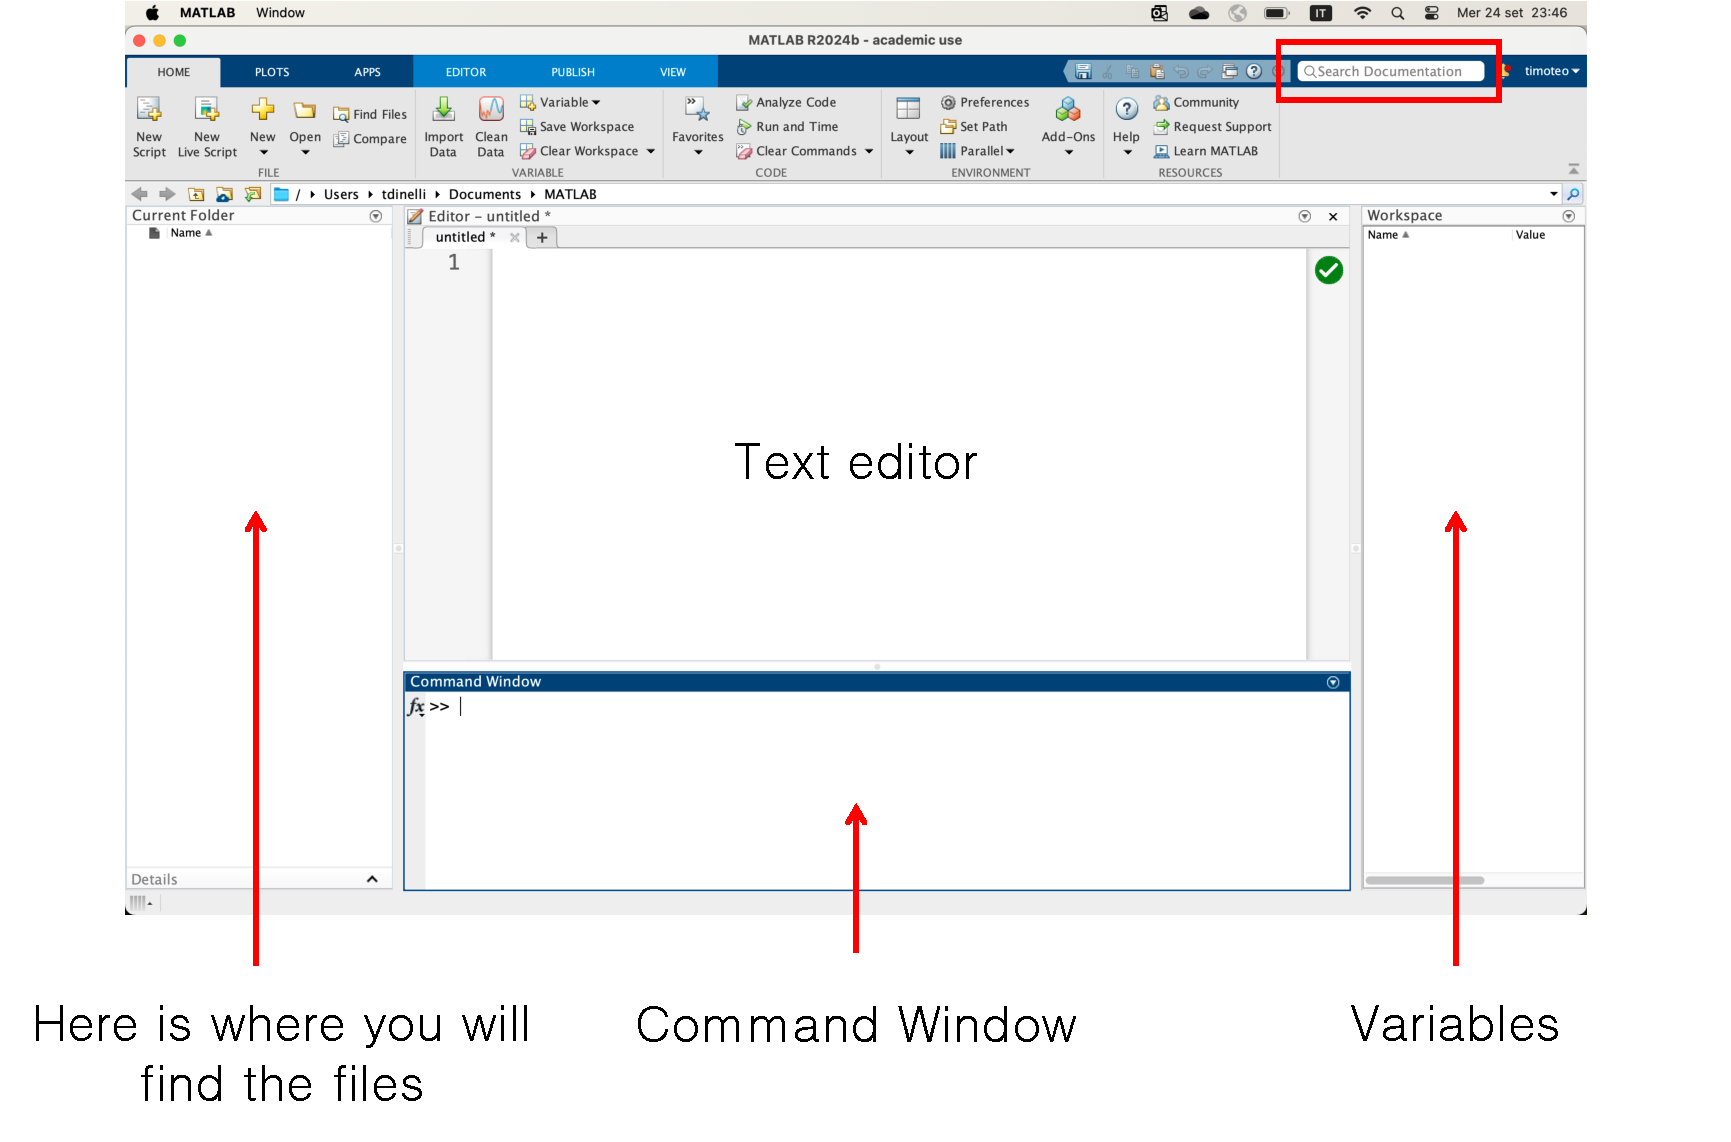
\includegraphics[width=0.8\textwidth]{figures/matlab.pdf}
    \end{figure}
\end{frame}

\begin{frame}{What can a Computer handle?}
    \begin{itemize}[<+->]
        \item[$\blacktriangleright$]
        MATLAB deals with numbers, arrays of numbers, characters, strings.
        
        \item[$\blacktriangleright$]
        Numbers can be of different types: signed and unsigned integers, and single-precision and double-precision floating-point numbers.
        
        \item[$\blacktriangleright$]
        When we set a variable value it gets stored as a series of 0 and 1 in a memory slot whose size depends on the type of variable (i.e., single-precision floating point numbers take 32 bits, or 4 bytes of memory, double precision 64 bit, or 8 bytes).
              
        \item[$\blacktriangleright$]
        By default, MATLAB store all values as double-precision floating point.
    \end{itemize}
\end{frame}

\subsection{Variables}
\begin{frame}[fragile]{Area of a cylinder}
    \large \textcolor{NavyBlue}{Let's compute the area of a cylinder given the diameter D = 20 cm and height h = 50 cm}.

    \vskip 1.cm
    \begin{columns}
        \begin{column}{0.5\textwidth}
            \textbf{Code:}
            \begin{minted}[frame=lines,framesep=2mm,numbersep=5pt,fontsize=\footnotesize,linenos]{octave}
D = 0.2;        % m (diameter)
h = 0.5;        % m (height)
perimeter = pi * D;
Area = perimeter * h;
            \end{minted}
        \end{column}
        \begin{column}{0.5\textwidth}
            \textbf{What happens:}
            \begin{enumerate}
                \item Create variable \texttt{D} = 0.2 m
                \item Create variable \texttt{h} = 0.5 m
                \item Calculate \texttt{perimeter} = $\pi \times 0.2$
                \item Calculate \texttt{Area} = perimeter $\times$ 0.5
            \end{enumerate}
        \end{column}
    \end{columns}
\end{frame}

\begin{frame}[fragile]{Source code: scripts and functions in MATLAB}
    Scripts are m-files (text format) containing MATLAB statements. MATLAB ``functions'' are another type of m-file. The biggest difference between scripts and functions is that functions have input and output parameters. Script files can only operate on the variables that are ``hard-coded'' into their m-file.

    \begin{columns}[T]
    \column{0.45\textwidth}
    \begin{minted}[frame=lines,framesep=2mm,numbersep=5pt,fontsize=\footnotesize,linenos]{octave}
D = 0.2;        % m
h = 0.5;        % m
perimeter = pi * D;
Area = perimeter * h;
    \end{minted}
    \vspace{2mm}
    \texttt{ans = 0.3142}
    
    \column{0.55\textwidth}
    \begin{minted}[frame=lines,framesep=2mm,numbersep=5pt,fontsize=\footnotesize,linenos]{octave}
function Area = ComputeArea(D, h)
    perimeter = pi * D;
    Area = perimeter * h;
end
    \end{minted}
    \vspace{2mm}
    \begin{minted}[frame=lines,framesep=2mm,numbersep=5pt,fontsize=\footnotesize]{octave}
ComputeArea(0.2, 0.5)
    \end{minted}
    \texttt{ans = 0.3142}
\end{columns}
\end{frame}

\begin{frame}{Variables names}
    \begin{itemize}
        \item[$\blacktriangleright$]
        MATLAB is case sensitive! \textbf{Pippo $\neq$ pippo}

        \item[$\blacktriangleright$]
        Variables name should be self explanatory, so prefer \textbf{distance, radius, ...} than \textbf{a, b, ...}

        \item[$\blacktriangleright$]
        When possible \underline{\textbf{use}} the camel case notation to make stuff easier to read. \textbf{PipeLength, GasTemperature, ...}.
    \end{itemize}
\end{frame}
 
\subsection{Arrays and Matrices}
\begin{frame}[fragile]{Arrays and Matrices}
    % \vskip -.5cm
    \begin{itemize}
        \item[$\blacktriangleright$]
        In MATLAB \textbf{arrays} are defined as:
        \begin{minted}[frame=lines,framesep=2mm,numbersep=5pt,fontsize=\footnotesize]{octave}
v = [5 13 97 31 98]
        \end{minted}
        %\vspace{2mm}
        \texttt{v =} \\
        \texttt{\hspace{3em} 5 \hspace{3em} 13 \hspace{3em} 97 \hspace{3em} 31 \hspace{3em} 98}

        \item[$\blacktriangleright$]
        \textbf{Matrices} can be defined as a set of stacked arrays separated with ;
        \begin{minted}[frame=lines,framesep=2mm,numbersep=5pt,fontsize=\footnotesize]{octave}
M = [5 13 97; 31 98 36; 11 9 20]
        \end{minted}
        \vspace{2mm}
        \texttt{M =} \\
        \texttt{\hspace{3em} 5 \hspace{3em} 13 \hspace{3em} 97} \\
        \texttt{\hspace{3em} 31 \hspace{3em}98 \hspace{3em} 36} \\
        \texttt{\hspace{3em} 11 \hspace{3em} 9 \hspace{3em} 20}
    \end{itemize}
\end{frame}

\begin{frame}[fragile]{}
    \begin{itemize}
        \item[$\blacktriangleright$]
        Elements can be accessed using their index (indices in MATLAB starts from 1)
        \begin{minted}[frame=lines,framesep=2mm,numbersep=5pt,fontsize=\footnotesize]{octave}
v(1)
        \end{minted}
        \vspace{2mm}
        \texttt{ans = 5}

        \begin{minted}[frame=lines,framesep=2mm,numbersep=5pt,fontsize=\footnotesize]{octave}
M(2,1)  % (row number, column number)
        \end{minted}
        \vspace{2mm}
        \texttt{ans = 31}
    \end{itemize}
\end{frame}
 
\begin{frame}[fragile]{Creating arrays and matrices}
    \begin{itemize}
        \item[$\blacktriangleright$]
        Create a matrix of zeros or ones:
        \begin{columns}[T]
            \column{0.5\textwidth}
            \begin{minted}[frame=lines,framesep=2mm,numbersep=5pt,fontsize=\footnotesize]{octave}
A = zeros(3,2)
            \end{minted}
            \vspace{2mm}
            \texttt{A =} \\
            \texttt{\hspace{3em} 0 \hspace{3em} 0} \\
            \texttt{\hspace{3em} 0 \hspace{3em} 0} \\
            \texttt{\hspace{3em} 0 \hspace{3em} 0}
        
            \column{0.5\textwidth}
            \begin{minted}[frame=lines,framesep=2mm,numbersep=5pt,fontsize=\footnotesize]{octave}
A = ones(2,3)
            \end{minted}
            \vspace{2mm}
            \texttt{A =} \\
            \texttt{\hspace{3em} 1 \hspace{3em} 1 \hspace{3em} 1} \\
            \texttt{\hspace{3em} 1 \hspace{3em} 1 \hspace{3em} 1}
        \end{columns}
    \end{itemize}
\end{frame}
 
\begin{frame}[fragile]{}
    \begin{itemize}
        \item[$\blacktriangleright$]
        Create a vector of \textbf{n} equally spaced elements:
        \begin{minted}[frame=lines,framesep=2mm,numbersep=5pt,fontsize=\footnotesize]{octave}
v1 = [1:2:11]  % Parenthesis can be omitted
        \end{minted}
        \vspace{2mm}
        \texttt{v1 = \hspace{2em} 1 \hspace{2em} 3 \hspace{2em} 5 \hspace{2em} 7 \hspace{2em} 9 \hspace{2em} 11}
        \vspace{4mm}
        
        \begin{minted}[frame=lines,framesep=2mm,numbersep=5pt,fontsize=\footnotesize]{octave}
v2 = [1:3:11]  % Parenthesis can be omitted
        \end{minted}
        \vspace{2mm}
        \texttt{v2 = \hspace{2em} 1 \hspace{2em} 4 \hspace{2em} 7 \hspace{2em} 10 \hspace{1.em} \alert{\% be careful!}} \\
        \vspace{2mm}

        \begin{minted}[frame=lines,framesep=2mm,numbersep=5pt,fontsize=\footnotesize]{octave}
v3 = linspace(1,10,6)  % Parenthesis can NOT be omitted!
        \end{minted}
        \vspace{2mm}
        \texttt{v3 = \hspace{2em} 1.0 \hspace{2em} 2.8 \hspace{2em} 4.6 \hspace{2em} 6.4 \hspace{2em} 8.2 \hspace{2em} 10.0}
    \end{itemize}
\end{frame}
 
\begin{frame}[fragile]{Operations with arrays and matrices}
    \begin{columns}
    \column{0.5\textwidth}
    \begin{itemize}
        \vspace{-22pt}
        \item[$\blacktriangleright$]
        Size of a matrix:
        \begin{minted}[frame=lines,framesep=2mm,numbersep=5pt,fontsize=\footnotesize]{octave}
M = [1 2 3; 4 5 6]
size(M)
        \end{minted}
        \texttt{ans = 2 3}

        \item[$\blacktriangleright$]
        Copying a matrix:
        \begin{minted}[frame=lines,framesep=2mm,numbersep=5pt,fontsize=\footnotesize]{octave}
A = M
        \end{minted}
        \texttt{A =} \\
        \texttt{\hspace{3em} 1 \hspace{3em} 2 \hspace{3em} 3} \\
        \texttt{\hspace{3em} 4 \hspace{3em} 5 \hspace{3em} 6}
    \end{itemize}
    \column{0.5\textwidth}
    \begin{itemize}
        \vspace{-15pt}
        \item[$\blacktriangleright$]
        Copying a line or a column of a matrix:
        \begin{minted}[frame=lines,framesep=2mm,numbersep=5pt,fontsize=\footnotesize]{octave}
v = M(1,:)
        \end{minted}
        \texttt{v =} \\
        \texttt{\hspace{3em} 1 \hspace{3em} 2 \hspace{3em} 3}

        \item[$\blacktriangleright$]
        Size of an array:
        \begin{minted}[frame=lines,framesep=2mm,numbersep=5pt,fontsize=\footnotesize]{octave}
size(v)
        \end{minted}
        \texttt{ans = 1 3}

        \begin{minted}[frame=lines,framesep=2mm,numbersep=5pt,fontsize=\footnotesize]{octave}
length(v)
        \end{minted}
        \texttt{ans = 3}
    \end{itemize}
    \end{columns}
\end{frame}
 
\begin{frame}[fragile]{}
    \begin{columns}
        \column{0.5\textwidth}
        \begin{itemize}
            \item[$\blacktriangleright$]
            Matrix transposition:
            \begin{minted}[frame=lines,framesep=2mm,numbersep=5pt,fontsize=\footnotesize]{octave}
C = B'
            \end{minted}
            \texttt{C =} \\
            \texttt{\hspace{3em} 1 \hspace{3em} 4} \\
            \texttt{\hspace{3em} 2 \hspace{3em} 5} \\
            \texttt{\hspace{3em} 3 \hspace{3em} 6}

            \item[$\blacktriangleright$]
            Element wise multiplication:
            \begin{minted}[frame=lines,framesep=2mm,numbersep=5pt,fontsize=\footnotesize]{octave}
M .* M
            \end{minted}
            \texttt{ans =} \\
            \texttt{\hspace{3em} 1  \hspace{3em} 4  \hspace{3em} 9} \\
            \texttt{\hspace{3em} 16 \hspace{3em}25 \hspace{3em} 36}
        \end{itemize}

        \vspace{-10pt}
        \column{0.5\textwidth}
        \begin{itemize}
            \item[$\blacktriangleright$]
            Matrix multiplication:
            \begin{minted}[frame=lines,framesep=2mm,numbersep=5pt,fontsize=\footnotesize]{octave}
M * B
            \end{minted}
            \textcolor{red}{\small{Error using * Inner matrices dimensions must agree.}} \\

            \begin{minted}[frame=lines,framesep=2mm,numbersep=5pt,fontsize=\footnotesize]{octave}
M * C
            \end{minted}
            \texttt{ans =} \\
            \texttt{14 \hspace{3em}32} \\
            \texttt{32 \hspace{3em}77} \\
            \vspace{5pt}
            \alert{N.B.} \footnotesize{\texttt{size(M) = 2 3; size(C) =  3 2}}
        \end{itemize}
    \end{columns}
\end{frame}

% ==================================================================
% PART 2
{
    \setbeamertemplate{footline}{}
    \begin{frame}[standout]
        Loops and conditional statements
    \end{frame}
}
\begin{frame}[fragile]{\textcolor{blue}{for} loop}
    \begin{itemize}
        \item[$\blacktriangleright$]
        The \textbf{for} loop repeats a series of instructions a
        \alert{fixed number of times}.
        \begin{minted}[frame=lines,framesep=2mm,numbersep=5pt,fontsize=\footnotesize,linenos]{octave}
for i = 1:10
    paperino(i) = i;
end
        \end{minted}
        \texttt{paperino = 1} \\
        \texttt{paperino = 1 2} \\
        \texttt{paperino = 1 2 3} \\
        \texttt{...} \\
        \texttt{paperino = 1 2 3 4 5 6 7 8 9} \\
        \texttt{paperino = 1 2 3 4 5 6 7 8 9 10}
    \end{itemize}
\end{frame}

\begin{frame}[fragile]{}
    \begin{itemize}
        \item[$\blacktriangleright$]
        The index of the \textbf{for} loop can be changed by an \alert{arbitrary increment}:
        \begin{minted}[frame=lines,framesep=2mm,numbersep=5pt,fontsize=\footnotesize,linenos]{octave}
for i = 10:-1:1
    pluto(i) = i;
end
        \end{minted}
        \texttt{pluto = 0 0 0 0 0 0 0 0 0 10} \\
        \texttt{pluto = 0 0 0 0 0 0 0 0 9 10} \\
        \texttt{pluto = 0 0 0 0 0 0 0 8 9 10} \\
        \texttt{...} \\
        \texttt{pluto = 0 2 3 4 5 6 7 8 9 10} \\
        \texttt{pluto = 1 2 3 4 5 6 7 8 9 10}
    \end{itemize}
\end{frame}

\begin{frame}[fragile]{Examples}
    \begin{itemize}
        \item[$\blacktriangleright$]
        Sum the first hundred natural numbers.
        \begin{equation*}
            \sum_{i = 1}^{100} i = ?.
        \end{equation*}
        
        \item[$\blacktriangleright$]
        Sum hundred times one.
        \begin{equation*}
            \sum_{i=1}^{100} 1 = ?
        \end{equation*}
        
        \begin{columns}
            \begin{column}{0.5\textwidth}
                \begin{minted}[frame=lines,framesep=2mm,numbersep=5pt,fontsize=\footnotesize,linenos]{octave}
sum = 0;
for i = 1:100
    sum = sum + i;
end
disp(sum);
                \end{minted}
            \end{column}
            \begin{column}{0.5\textwidth}
                \begin{minted}[frame=lines,framesep=2mm,numbersep=5pt,fontsize=\footnotesize,linenos]{octave}
sum = 0;
for i = 1:100
    sum = sum + 1;
end
disp(sum);
                \end{minted}
            \end{column}
        \end{columns}
    \end{itemize}
\end{frame}

\subsection{While}
\begin{frame}[fragile]{\textcolor{blue}{while} loop}
    \begin{itemize}
        \item[$\blacktriangleright$]
        The \textbf{while} loop repeats a series of instructions \alert{until a condition is TRUE}.

        \item[$\blacktriangleright$]
        N.B. pay attention with the while loop it can run till infinite, \alert{handle with care}.
    \end{itemize}
    \begin{minted}[frame=lines,framesep=2mm,numbersep=5pt,fontsize=\footnotesize,linenos]{octave}
result = 0;
token = 0;
while (sum < 325)
    token = token + 1;
    result = result + token;
end
disp(['Iteration number: ', num2str(token)]);
disp(['Sum is equal to:  ', num2str(result)]);
    \end{minted}
    \texttt{Iteration number: 25} \\
    \texttt{Sum is equal to: 325}
\end{frame}

\section{Conditional statements}
\subsection{If, else if, else}
\begin{frame}[fragile]{\textcolor{blue}{IF} Statement}
    \begin{itemize}
        \item[$\blacktriangleright$]
        The \textcolor{blue}{\textbf{IF}} statement executes a series of instructions only \textcolor{blue}{\textbf{IF}} a condition is TRUE:
    \end{itemize}

    \vspace{1.cm}
    \begin{columns}
        \column{0.5\textwidth}
        \begin{minted}[frame=lines,framesep=2mm,numbersep=5pt,fontsize=\footnotesize,linenos]{octave}
if (condition)
    % instructions
elseif (condition)
    % instructions
elseif (condition)
    % instructions
else
    % instructions
end
        \end{minted}
        \column{0.5\textwidth}
        \textcolor{NavyBlue}{\textbf{Example}: Write a simple script to compute the absolute value of a number.}
        \vspace{0.01cm}
        \begin{minted}[frame=lines,framesep=2mm,numbersep=5pt,fontsize=\footnotesize,linenos]{octave}
x = 35;
if (x >= 0)
    abs = x;
else
    abs = -x;
end
        \end{minted}
    \end{columns}
\end{frame}

\section{Functions}
\begin{frame}{Functions}
    In MATLAB, a \alert{function} is a block of code that takes inputs, performs a set of operations, and returns outputs. Functions allow you to organize code in a clearer and more reusable way, especially when you need to perform the same operation in different parts of your program.

    \textbf{Why using functions?}
    \begin{itemize}
        \item[$\blacktriangleright$] \textbf{Modularity}: Separating code into functions makes the program more readable and easier to maintain.

        \item[$\blacktriangleright$] \textbf{Reusability}: A function can be reused in different parts of the program without rewriting the code.
    \end{itemize}
\end{frame}

\begin{frame}[fragile]{Syntax}
    \begin{minted}[frame=lines,framesep=2mm,numbersep=5pt,fontsize=\footnotesize,linenos,escapeinside=||]{octave}
function |\tikzmark{out}|[y1, ..., yN] = |\tikzmark{name}|function_name|\tikzmark{inp}|(x1, ..., xM)
% ...
% ...
% ...
% Some code
% ...
% ...
% ...
end
    \end{minted}
    \begin{tikzpicture}[overlay, remember picture, >=stealth, nodes={align=left,inner ysep=1pt},<-]
        \node[anchor=west, color=RoyalPurple!85, yshift=-2em, xshift=5.2em] (inputtext) at (pic cs:inp)
        {\textsf{\footnotesize Input variables.}};
        \draw [color=RoyalPurple]([xshift=35pt,yshift=-0.3em]pic cs:inp) |- ([yshift=-0.2ex]inputtext.south east);
        
        \node[anchor=west, color=WildStrawberry!85, yshift=-4em, xshift=4em] (fnametext) at (pic cs:name)
        {\textsf{\footnotesize Name of the function (user defined).}};
        \draw [color=WildStrawberry]([yshift=-0.3em,xshift=35pt]pic cs:name) |- ([yshift=-0.2ex]fnametext.south east);
        
        \node[anchor=west, color=OliveGreen!85, yshift=-6em, xshift=7.5em] (outtext) at (pic cs:out)
        {\textsf{\footnotesize Output variables (parenthesis can be omitted).}};
        \draw [color=OliveGreen]([yshift=-0.3em,xshift=35pt]pic cs:out) |- ([yshift=-0.2ex]outtext.south east);
    \end{tikzpicture}
\end{frame}

\section{Exercises}
% \begin{frame}[fragile]{Example}
%     Let's define a square matrix populated with random numbers, using the function
%     \textbf{magic()} and loop over its rows and columns to match specific conditions.
% 
%     \begin{minted}[frame=lines,framesep=2mm,numbersep=5pt,fontsize=\footnotesize,linenos]{octave}
% clear, clc
% M = magic(300);
% for i = 1:300
%     for j = 1:300
%         if (M(i,j) == 569)
%             disp('Found!')
%         end
%     end
% end
%     \end{minted}
% \end{frame}

\begin{frame}{The Babylonian method}
    \textcolor{NavyBlue}{Let's write a script implementing the Babylonian method to compute the square root of a number with a precision of four decimal figures, then wrap this code into a function.}
    \begin{enumerate}
        \item \textbf{Make an Initial guess}.
              Guess any positive number $x_{0}$.
        \item \textbf{Improve the first guess}.
              Apply the formula $x_{1} = \frac{x_{0} + \frac{S}{x_{0}}}{2}$. The number $x_{1}$
              is a better approximation to $\sqrt{S}$.
        \item \textbf{Iterate until convergence}.
              Apply the formula $x_{n+1} = \frac{x_{n} + \frac{S}{x_{n}}}{2}$ until the
              convergence is reached.
    \end{enumerate}
    \textbf{Convergence} is reached when the digits of $x_{n+1}$ and $x_{n}$ agree to as many
    decimal places as you desire.
\end{frame}

\begin{frame}[fragile]{Implementation}
    \begin{minted}[frame=lines,framesep=2mm,numbersep=5pt,fontsize=\footnotesize,linenos]{octave}
function SquareRoot = ComputeSquareRoot(S)
    iter = 0;
    x0 = S;
    y = 0.5 * (x0 + S/x0);
    
    while abs(x0-y) > 1e-4 && iter < 50
        x0 = y;
        y = 0.5 * (x0 + S/x0);
        iter = iter + 1;
    end
    
    disp(['Number of iteration to reach convergence: ', num2str(iter)])
    SquareRoot = y;
end
    \end{minted}
\end{frame}

{
    \setbeamertemplate{footline}{}
    \begin{frame}[standout]
        Thank you for the attention!
    \end{frame}
}
\end{document}
